\documentclass[8pt,landscape]{article}

% PACKAGES
\usepackage[letterpaper, margin=0.1in]{geometry}
\usepackage{amsmath, amssymb, geometry}
\usepackage{multicol}
\usepackage{setspace}
\usepackage{sectsty}
\usepackage{verbatim}
\usepackage{graphicx}
\usepackage{xcolor}
\usepackage{listings}
\usepackage{enumitem}
\usepackage{booktabs} % For better tables if needed

% Define a custom color for code highlighting and environment
\definecolor{myred}{RGB}{204, 0, 0} % A strong red
\definecolor{mygray}{RGB}{240, 240, 240} % Light gray for background

% LISTINGS SETUP for R and Python
\lstset{
  basicstyle=\ttfamily\scriptsize\color{black}, % Tiny font for code
  backgroundcolor=\color{mygray},
  frame=single,
  frameround=tttt,
  framesep=3pt,
  rulesepcolor=\color{black!20},
  breaklines=true,
  columns=fullflexible,
  showstringspaces=false,
  commentstyle=\color{gray},
  keywordstyle=\color{blue!80!black},
  stringstyle=\color{myred}, % Use red for strings to match the custom \code{} style
  breakatwhitespace=true,
  xleftmargin=0pt,
  xrightmargin=0pt,
  aboveskip=0.5ex,
  belowskip=0.5ex
}

% FORMATTING
\setstretch{0.9} % Reduce line spacing
\setlength{\parindent}{0pt}
\setlength{\parskip}{0pt}

% Reduce section spacing and change color
\sectionfont{\fontsize{8}{9}\selectfont\bfseries\color{black}} % Main section font: 8pt
% Reduce subsection spacing and make subsections blue
\makeatletter
\renewcommand{\subsection}{\@startsection{subsection}{2}{0pt}%
    {0.1ex}% space before subsection
    {0.1ex}% space after subsection
    {\fontsize{8}{9}\bfseries\color{blue}}} % Subsection font: 8pt
\makeatother

% Custom command for red-highlighted code/commands (for in-line use)
\newcommand{\code}[1]{\textcolor{myred}{\texttt{#1}}}

% Custom small text wrapper - ensuring 8pt for body text
\newcommand{\smalltext}[1]{%
  {\fontsize{8}{9}\selectfont\sloppy #1\par}%
}

% DOCUMENT START
\begin{document}
\fontsize{8}{9}\selectfont % Set the base font size to 8pt and line skip to 9pt for the entire document
\pagestyle{empty}
\begin{multicols}{3}
\textbf{algorithm}: a well-defined computational procedure designed to solve a problem. It consists of a sequence of precise steps that take some inputs, process them systematically, and produce corresponding outputs. 
\textbf{data structure}: is a way to organize and manage data, allowing us to write more efficient code in terms of both time and space. 
\subsection{Big O Notation}
\smalltext{
\textbf{Definition}: Describes asymptotic behavior of algorithms as input size $n$ grows.
\textbf{Common Classes}:
\begin{itemize}[noitemsep, nolistsep, leftmargin=1em]
    \item $O(1)$: Constant - Runtime independent of $n$.
    \item $O(\log n)$: Logarithmic - Doubling $n$ adds constant time.
    \item $O(\sqrt{n})$: sub-linear time complexity.
    \item $O(n)$: Linear - Doubling $n$ doubles time.
    \item $O(n \log n)$: Linearithmic - Roughly $O(n)$ when $n$ doubles.
    \item $O(n^2)$: Quadratic - Doubling $n$ multiplies time by 4.
    \item $O(n^k)$: Polynomial - Time multiplied by $2^k$.
    \item $O(2^n)$: Exponential - Doubling $n$ multiplies time by $2^k$.
\end{itemize}
}
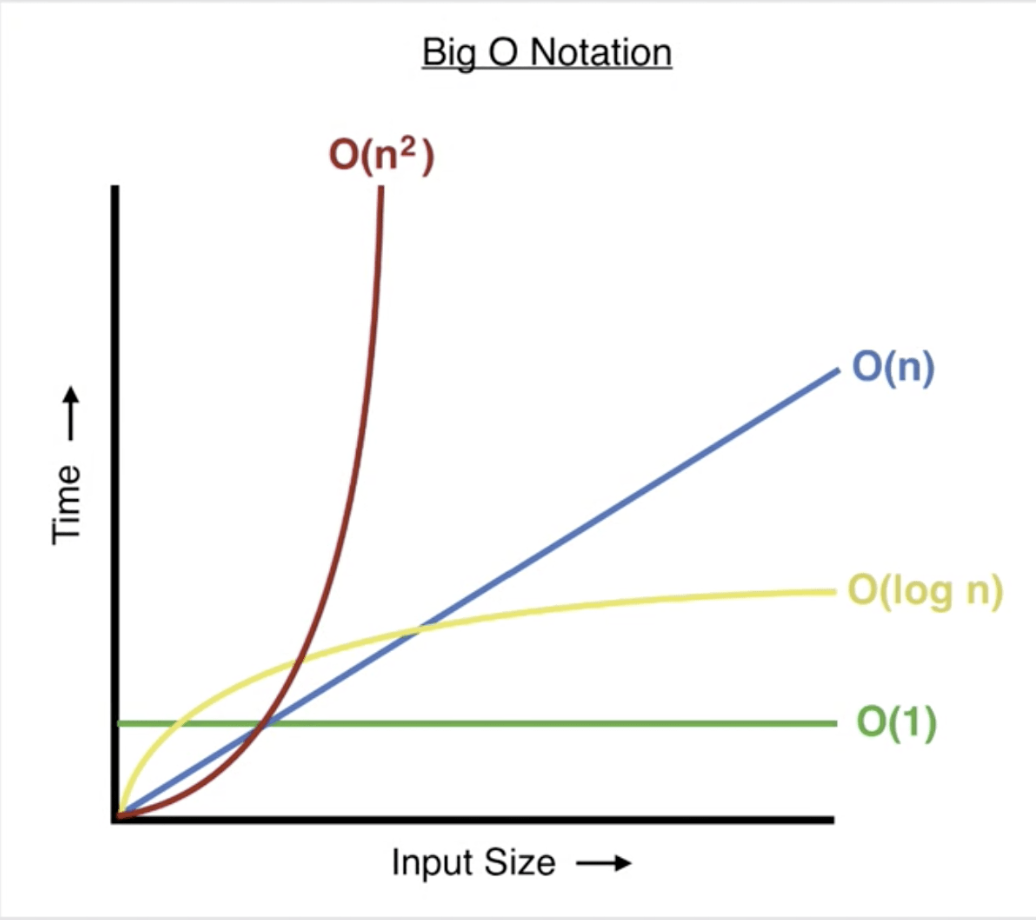
\includegraphics[width=0.7\linewidth]{img-1.png}
\subsection{Hash Tables}
\smalltext{
\textbf{Properties}: Keys must be \textbf{hashable} (immutable).
\textbf{Operations}:
\begin{itemize}[noitemsep, nolistsep, leftmargin=1em]
    \item $O(1)$ \code{insert}, \code{delete}, \code{lookup} (average).
\end{itemize}
\textbf{Hash Function}: Deterministic: same input $\to$ same output.
\textbf{Collisions}: Handled by \textbf{chaining} (list per bucket).
\textbf{Python Dict}:
\begin{itemize}[noitemsep, nolistsep, leftmargin=1em]
    \item Keys must be \textbf{hashable}.
    \item Values can be any type.
    \item Lists cannot be keys (mutable).
\end{itemize}
}

\subsection{Graphs}
\smalltext{
  For some graphs, DFS is equivalent to BFS. \\
  Represent a \textbf{2D image} having M rows and N columns using a graph \\
  Space Complexity is $MN^2$  in Adjacency Matrix\\
  Space Complexity is $MN$  in Adjacency List\\
\textbf{Definition}: $G=(V, E)$ where $V$=vertices, $E$=edges.
\textbf{Types}:
\begin{itemize}[noitemsep, nolistsep, leftmargin=1em]
    \item \textbf{Undirected}: edges have no direction (e.g., Twitter followers).
    \item \textbf{Directed}: edges \textbf{bidirectional} (e.g., Facebook friends).
    \item \textbf{Weighted}: edges have numerical values.
    \item \textbf{Unweighted}: edges represent presence/absence only.
\end{itemize}
\textbf{Adjacency List}: Array of lists: $Adj[u]$ is a list of neighbors of $u$.
\begin{itemize}[noitemsep, nolistsep, leftmargin=1em]
    \item Space: $O(V+E)$.
    \item Good for \textbf{sparse graphs} ($E \ll V^2$).
    \item Lookup time: $O(V)$ worst case.
\end{itemize}
\textbf{Adjacency Matrix}: A matrix where $A[i][j]=1$ if edge exists.
\begin{itemize}[noitemsep, nolistsep, leftmargin=1em]
    \item Space: $O(V^2)$.
    \item Lookup time: $O(1)$.
    \item Good for \textbf{dense graphs}.
\end{itemize}
}

\subsection{Breadth-First Search (BFS)}
\smalltext{
\textbf{Purpose}: Explores neighbors before going deeper. Finds shortest paths in unweighted graphs.
\textbf{Data Structure}: Uses \textbf{Queue} (FIFO).
\textbf{Complexity}: $O(V+E)$.
\textbf{Implementation}:
\begin{enumerate}[noitemsep, nolistsep, leftmargin=1em]
    \item Initialize stack with start node.
    \item Mark start as \textbf{visited}.
    \item While stack not empty:
    \item \hspace{0.5em}- Pop node. \#stack.pop(0) in Queue
    \item \hspace{0.5em}- Process node.
    \item \hspace{0.5em}- Enqueue unvisited neighbors.
    \item \hspace{0.5em}- Mark neighbors as \textbf{visited}.
\end{enumerate}
}
\begin{lstlisting}[language=Python]
# --- Option 1: Built-in BFS traversal ---
print("BFS traversal using networkx.bfs_tree:")
bfs_tree = nx.bfs_tree(G, source='A')
print(list(bfs_tree.nodes()))  # nodes in BFS order
# OR equivalently:
print("\nUsing networkx.bfs_edges:")
bfs_edges = list(nx.bfs_edges(G, source='A'))
print("BFS edges:", bfs_edges)
# --- Option 2: Custom BFS implementation ---
def bfs_custom(G, start):
    visited = set()
    queue = deque([start])
    while queue:
        node = queue.popleft()
        if node not in visited:
            print(node, end=" ")
            visited.add(node)
            for neighbor in G.neighbors(node):
                if neighbor not in visited:
                    queue.append(neighbor)
    return visited
\end{lstlisting}

\subsection{Depth-First Search (DFS)}
\smalltext{
\textbf{Purpose}: Explores as deep as possible before backtracking.
\textbf{Data Structure}: Uses \textbf{Stack} (LIFO).
\textbf{Complexity}: $O(V+E)$.
\textbf{Implementation}:
\begin{enumerate}[noitemsep, nolistsep, leftmargin=1em]
    \item Initialize stack with start node.
    \item Mark start as \textbf{visited}.
    \item While stack not empty:
    \item \hspace{0.5em}- Pop node. \#stack.pop() in Queue
    \item \hspace{0.5em}- Process node.
    \item \hspace{0.5em}- Push unvisited neighbors.
    \item \hspace{0.5em}- Mark neighbors as \textbf{visited}.
\end{enumerate}
}
\begin{lstlisting}[language=Python]
# --- Option 2: Custom DFS using recursion ---
def dfs_recursive(G, node, visited=None):
    if visited is None:
        visited = set()
    visited.add(node)
    print(node, end=" ")
    for neighbor in G.neighbors(node):
        if neighbor not in visited:
            dfs_recursive(G, neighbor, visited)
    return visited
print("\nCustom DFS (recursive):")
dfs_recursive(G, 'A')
# --- Option 3: Iterative DFS using a stack ---
def dfs_iterative(G, start):
    visited = set()
    stack = [start]
    while stack:
        node = stack.pop()
        if node not in visited:
            print(node, end=" ")
            visited.add(node)
            # Add neighbors to stack
            stack.extend(reversed(list(G.neighbors(node))))
    return visited
\end{lstlisting}

\subsection{Sparse Matrix format (Scipy)}
\smalltext{
  This is “Compressed Sparse Row” format. \\
  It means we store an adjacency list per row. \\
  Sparse matrices come up a lot in practice, beyond just adjacency matrices in graphs. For example: \\
Word counts: We might represent a document by the words in it, but only a small fraction of all words would appear in a given document. \\
Ratings: We might represent an Amazon item by the user ratings, but only a small fraction of all users have rated a given item. \\
}

\subsection{Sparse Matrix Formats}
\smalltext{
\textbf{Compressed Sparse Row (CSR) vs. Column (CSC)}
}
\centering
\begin{tabular}{p{1.4cm} p{1.6cm} p{1.6cm}}
\toprule
\textbf{Feature} & \textbf{CSR} & \textbf{CSC} \\
\midrule
Storage Arrays & Values, Column Indices, Row Pointers & Values, Row Indices, Column Pointers \\
Optimized For & Row operations & Column operations \\
Access Pattern & Fast row slicing & Fast column slicing \\
Use Cases & Matrix-vector multiplication, row-wise operations & Column-wise computations, matrix factorization \\
\bottomrule
\end{tabular}
\smalltext{
CSR and CSC are efficient ways to store matrices with mostly zero entries, saving memory and speeding up relevant operations.
}

\begin{lstlisting}[language=Python]
x = scipy.sparse.random(5, 5, density=0.2, format="csr", random_state=321)

\end{lstlisting}


\subsection{Trees}
\smalltext{
Trees are vital for organizing data \textbf{hierarchically} (parent-child relationships).
\textbf{Modeling Real-World Systems}:
\begin{itemize}[noitemsep, nolistsep, leftmargin=1em]
    \item \textbf{File Systems} (folders/subfolders).
    \item \textbf{Organization Charts} (manager-employee).
    \item \textbf{XML/HTML Documents} (nested tags).
\end{itemize}
\textbf{Efficiency \& Algorithms}:
\begin{itemize}[noitemsep, nolistsep, leftmargin=1em]
    \item \textbf{Binary Search Trees (BSTs)}: Fast $O(\log n)$ average time for lookup/insertion/deletion.
    \item \textbf{Balanced Trees} (AVL/Red-Black): Consistently fast performance.
    \item \textbf{Heaps}: Used for Priority Queues and \code{heapsort}.
\end{itemize}
\textbf{Advanced Structures \& Applications}:
\begin{itemize}[noitemsep, nolistsep, leftmargin=1em]
    \item \textbf{Tries}: Autocomplete, spell checking.
    \item \textbf{Syntax Trees}: Compilers/interpreters.
    \item \textbf{B-Trees} / \textbf{B+ Trees}: Database indexing, file systems.
    \item \textbf{Decision Trees}: Machine learning models (random forests).
\end{itemize}
}
\subsection{Tree Terminology}
\smalltext{
\textbf{Node}: Fundamental part, stores data.
\textbf{Root}: The first node in a tree (no parent).
\textbf{Edge}: A link connecting two nodes.
\textbf{Parent}: Immediate predecessor (a node has only one parent).
\textbf{Child}: Immediate successor (a node can have $\geq 0$ children).
\textbf{Leaf Node}: A node with zero children.
\textbf{Height}: Maximum number of edges from the \textbf{root} to a \textbf{leaf node}.
\textbf{Subtree}: A portion of a tree starting from any node and including all its descendants.
\textbf{Balanced Tree}: A tree where the height of the left and right subtrees of any node are nearly equal.
}

\subsection{NetworkX Code Examples}
\smalltext{
\textbf{Create Graphs}:
\begin{itemize}[noitemsep, nolistsep, leftmargin=1em]
    \item \code{G = nx.Graph()} (undirected)
    \item \code{G = nx.DiGraph()} (directed)
\end{itemize}
\textbf{Add Nodes \& Edges}:
\begin{itemize}[noitemsep, nolistsep, leftmargin=1em]
    \item \code{G.add\_node("A")}
    \item \code{G.add\_edge("A", "B")}
    \item \code{G.add\_edges\_from([("A", "B"), ("B", "C"), ("B", "D")])}
\end{itemize}
}

\subsection{Time Measurement}
\smalltext{
\textbf{Code Profiling}:
\begin{itemize}[noitemsep, nolistsep, leftmargin=1em]
    \item \code{timeit}: Python magic for timing small code snippets.
    \item \code{line\_profiler}: Per-line timing.
\end{itemize}
\textbf{Memory Profiling}:
\begin{itemize}[noitemsep, nolistsep, leftmargin=1em]
    \item \code{sys.getsizeof()}: Object size.
    \item \code{df.memory\_usage()}: Pandas DataFrame memory.
    \item \code{np.sum(array.nbytes)}: NumPy arrays memory.
\end{itemize}
}

\subsection{Tips \& Best Practices}
\smalltext{
\textbf{Visualization}:
\begin{itemize}[noitemsep, nolistsep, leftmargin=1em]
    \item \code{nx.draw(G, with\_labels=True)}
\end{itemize}
\textbf{General Tips}:
\begin{itemize}[noitemsep, nolistsep, leftmargin=1em]
    \item Use \textbf{set} for membership lookup.
    \item Use \textbf{dict} for fast key-value lookups.
    \item Prioritize coherent \textbf{data structure} operations based on needs.
    \item Consider \textbf{space-time tradeoffs}.
    \item BFS is better for optimizing \textbf{shortest paths} in unweighted graphs.
    \item \textbf{Hash table operations} are $O(1)$ avg., not worst-case.
    \item Prefer \textbf{sparse matrices} for graphs with $E \ll V^2$.
\end{itemize}
}



\end{multicols}
\end{document}